\clearpage

\section{Bob QKD}

\maketitle
This block is the main processor for Alice. 

AliceQKD is a superblock intended work as Bob's main processor. It performs a 
series of functions, including classical channel communication with Alice and 
data processing for basis reconciliation, error correction and privacy 
amplification.

\subsection*{Input Parameters}

	\begin{itemize}
		\item
		\item
		
	\end{itemize}

\subsection*{Methods}



\subsection*{Functional description}
\begin{figure}[H]
	\centering
	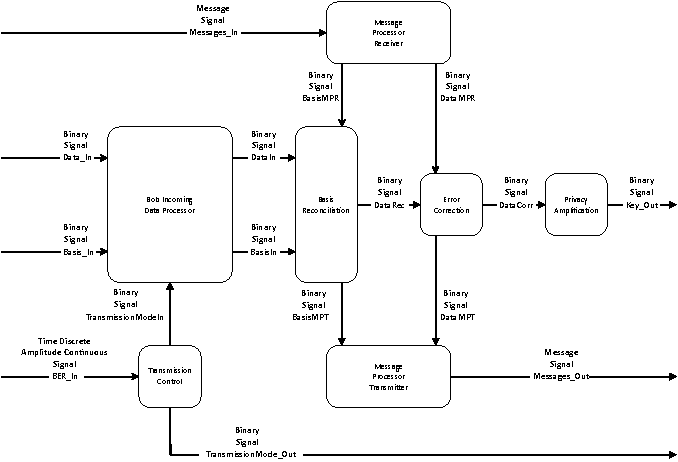
\includegraphics{./lib/bob_qkd2/figures/BobQKD_blockDiagram.pdf}
\end{figure}

BobQKD is a superblock intended to do classical channel communication and 
data processing  as required by the BB84 protocol. This superblock requires 
four different inputs:

\begin{itemize}
	\item Messages from Aliec, which are used to coordinate the required data 
	processing for key extraction;
	\item A binary signal corresponding to the measured trasmitted data;
	\item A binary signal corresponding to the basis used by Bob for 
	decoding the data sent by Alice.
	\item A continuous amplitude signal of the estimated Bit Error Rate, which is 
	used to control the transmission process. 
\end{itemize}

In addition, this block produces a total of three output signals:

\begin{itemize}
	\item	Messages intended to be read by Alice, used to coordinate the required 
	data processing for key extraction;
	\item A binary signal with the generated key;
	\item A binary signal corresponding to the transmission mode sent out.
\end{itemize}

The process inside the superblock is as follows:

The incoming BER signal is analyzed at the \textit{TransmissionControl} block. 
If the BER is too high, the process stops

The incoming data and basis signals are received in the 
\textit{BobIncomingDataProcessor} block. If the transmission is enabled, the 
incoming data and basis are sent into the \textit{BasisReconciliation} block


The \textit{BasisReconciliation} block in BobQKD is configured to start the 
basis reconciliation process. Thus, when enough samples are available, Bob 
sends a signal with the list of used basis to the 
\textit{MessageProcessorTransmitter} block. The block then waits.
When Alice responds, a message arrives at the \textit{MessageProcessorReceiver} 
block. It contains a binary string indicating whether Bob used the correct 
basis or not. This information is then sent to the \textit{BasisReconciliation} 
block. There, the bits where Bob got the right basis are sent to the 
\textit{ErrorCorrection} block, while the remaining ones are promptly discarded.


The \textit{ErrorCorrection} block will be responsible for correcting any 
errors that occurred during transmission. Similarly to the 
\textit{BasisReconciliation} block, in BobQKD it is configured to start acting 
when enough samples are available. When this condition is verified, the 
\textit{ErrorCorrection} block starts the Cascade process by dividing the 
available bits in segments, calculating their parities and sending them to the 
\textit{MessageProcessorTransmitter}. Once this is done, it waits until a 
response from Alice arrives at \textit{MessageProcessorReceiver}. The message 
should contain a reponse to Bob on whether the parities are similar or not. The 
Cascade process continues until it is concluded. The Cascade process is 
explained in the section of the \textit{ErrorCorrection} block, but is not 
fundamental to understanding the BobQKD superblock.

When the cascade process ends, the corrected data is output to the 
\textit{PrivacyAmplification} block, which does the necessary transformation to 
ensure the information that any attacker might have gained (Eve) is nullified.

The end result, and final output of the superblock, is a secure key 
shared known only to Alice and Bob.

\subsection*{Input Signals}


\subsection*{Examples}


\subsection*{Sugestions for future improvement} 